\section*{CHƯƠNG 1: GIỚI THIỆU}
\addcontentsline{toc}{section}{\numberline {} CHƯƠNG 1: GIỚI THIỆU}
\setcounter{section}{1}
\setcounter{figure}{0}
\subsection{TỔNG QUAN}
\subsubsection{Đặt vấn đề}
IoT (Internet of things) được dịch sang tiếng Việt với nhiều tên gọi khác nhau như Internet Vạn Vật, Mạng lưới thiết bị kết nối Internet, Mạng lưới vạn vật kết nối Internet,… Trong đó, thuật ngữ được sử dụng phổ biến nhất là Internet Vạn Vật.\\
\indent IoT là một liên mạng với sự tham gia của nhiều thành phần. Trong đó, các thiết bị, phương tiện sẽ được bổ sung và tích hợp thêm các bộ phận điện tử, phần mềm cũng như các loại cảm biến giúp chúng vừa có thể thu thập dữ liệu, vừa có thể kết nối qua mạng máy tính để truyền và chia sẻ các dữ liệu đó. Hệ thống các thiết bị, phương tiện thông minh này sẽ tạo nên một cơ sở hạ tầng đáp ứng nhu cầu phát triển của xã hội thông tin.\\
\indent IoT là công nghệ đóng vai trò quan trọng và bắt đầu tác động đến nhiều lĩnh vực và ngành công nghiệp, từ sản xuất, y tế, truyền thông, năng lượng cho đến ngành nông nghiệp. IoT bao gồm cơ sở hạ tầng truyền thông cơ bản được sử dụng để kết nối các đối tượng thông minh từ cảm biến, phương tiện, thiết bị di động đến việc thu thập dữ liệu từ xa dựa trên phân tích thông minh, giao tiếp người dùng và cách mạng hóa ngành nông nghiệp.\\
\indent Bằng cách triển khai các công nghệ cảm biến và IoT trong thực tiễn nông nghiệp đã làm thay đổi mọi khía cạnh của phương pháp canh tác truyền thống. IoT giúp cải thiện các giải pháp về canh tác truyền thống như ứng phó với hạn hán, tối ưu hóa năng suất, tính phù hợp đất đai, tưới tiêu và kiểm soát dịch hại.\\
\indent MQTT (Đầy đủ là Message Queuing Telemetry Transport) là một giao thức gửi tín hiệu dạng publish/subscribe. Chúng được sử dụng cho các thiết bị Internet of Things – IoT. Tín hiệu truyền đi với băng thông thấp, có độ tin cậy cao và khả năng sử dụng được trong mạng lưới thiếu ổn định. Bởi vì giao thức MQTT này sử dụng băng thông khá thấp trong môi trường có độ trễ cao nên nó là một giao thức lý tưởng cho các ứng dụng M2M (Machine to Machine).\\
\indent Công nghệ LoRa , được phát triển bởi Semtech , là một giao thức không dây mới được thiết kế để truyền thông tầm xa, năng lượng thấp. Giao thức cung cấp loại khả năng liên lạc mà các thiết bị thông minh cần có, và Liên minh LoRa đang hoạt động để đảm bảo khả năng tương tác giữa nhiều mạng trên toàn quốc.\\
\indent Một phần của phổ LoRa sử dụng thể hiện ít nhiễu điện từ, do đó tín hiệu có thể kéo dài một khoảng cách xa, thậm chí đi qua các tòa nhà, với rất ít năng lượng. Điều này phù hợp với các thiết bị IoT với dung lượng pin hạn chế. Điều đó cũng có nghĩa là các tinh thể chi phí thấp hơn có thể được sử dụng, do đó, việc xây dựng LoRa thành các thiết bị rẻ hơn.\\
\indent Mỗi gateway LoRa có thể xử lý hàng triệu node. Điều đó, cộng với thực tế là các tín hiệu có thể kéo dài khoảng cách đáng kể, có nghĩa là cần ít cơ sở hạ tầng mạng hơn, do đó làm cho việc xây dựng mạng LoRa rẻ hơn. Các mạng LoRa có thể được đặt cùng với các thiết bị liên lạc khác, như các tháp điện thoại di động, làm giảm đáng kể các hạn chế xây dựng.\\
\indent Các tính năng khác của LoRa cũng khiến nó trở nên lý tưởng cho IoT. LoRa sử dụng thuật toán tốc độ dữ liệu thích ứng để giúp tối đa hóa tuổi thọ pin và dung lượng mạng của thiết bị. Các giao thức của nó bao gồm nhiều lớp mã hóa, ở cấp độ mạng, ứng dụng và thiết bị, cho phép liên lạc an toàn. Tính hai chiều của giao thức hỗ trợ các thông điệp quảng bá, cho phép chức năng cập nhật phần mềm.\\
\indent Sự phát triển của Internet of Things bị giới hạn bởi dung lượng của mạng, bởi khả năng hoạt động của thiết bị mà không cần thay pin và bởi khả năng mã hóa truyền dẫn bí mật. Các tính năng được tích hợp trong LoRa cung cấp tất cả các khả năng này và sẽ cho phép sự phát triển rộng rãi của IoT.\\
\indent Với công nghệ Lora , chúng ta có thể truyền dữ liệu với khoảng cách lên hàng km mà không cần các mạch khuếch đại công suất; từ đó giúp tiết kiệm năng lượng tiêu thụ khi truyền/nhận dữ liệu. Do đó, LoRa có thể được áp dụng rộng rãi trong các ứng dụng thu thập dữ liệu như sensor network trong đó các sensor node có thể gửi giá trị đo đạc về trung tâm cách xa hàng km và có thể hoạt động với battery trong thời gian dài trước khi cần thay pin.\\
\\

\indent Nhận thấy những ưu điểm của Lora, giao thức MQTT và những ứng dụng vô cùng thực tế của IoT trong nông nghiệp. Chính vì vậy mục tiêu của đề tài tạo ra mạng kết nối với các thiết bị dùng để điều khiển, các cảm biến thu thập dữ liệu, vẽ đồ thị trạng thái dựa trên dữ liệu thu thập được từ cảm biến thông qua mạng LoRa và giao thức MQTT.
\subsubsection{Hiện trạng nông nghiệp Việt Nam}
\textbf{\textit{Cơ hội và thách thức}}\\
\indent Điều kiện tự nhiên và vị trí địa lý ưu ái cho nền nông nghiệp Việt Nam với nguồn nước tưới dồi dào, đa dạng các loại cây trồng và vật nuôi. Tuy vậy, cũng gặp không ít khó khăn như: thiên tai, bão lũ, xâm nhập mặn,... Đồng bằng sông Cửu Long là ngõ giao thương quan trọng trên thế giới, là nơi trung chuyển hàng hóa đi Châu Á Thái Bình Dương.\\
\indent Vào thời hội nhập, thị trường thế giới được mở rộng cùng những thay đổi cơ cấu từ sản xuất cây lương thực sang cây rau màu và thủy sản. Người tiêu dùng có xu hướng sử dụng các sản phẩm hữu cơ, thân thiện với môi trường. Thị trường xuất khẩu nông sản Việt Nam tiềm năng nhưng rủi ro cao khi giá cả nông sản trên thế giới thay đổi bất thường.\\
\indent Hiệp định tự do hóa thương mại lớn như CPTPP và EVFTA tạo cơ hội cho nông sản Việt Nam tiếp cận với thị trường thế giới. Tuy nhiên, cũng sẽ tạo ra khó khăn không nhỏ về cam kết sâu rộng và cáo buộc cao. Chất lượng nông sản và việc truy xuất nguồn gốc nông sản là một khó khăn lớn với nền nông nghiệp Việt Nam.\\
\indent \textbf{\textit{Thành tựu nông nghiệp Việt Nam}}\\
\indent Trong năm 2019, các mặt hàng như: gỗ, tôm, rau quả và hạt điều có kim ngạch xuất khẩu trên 3 tỷ USD trong nhóm 8 mặt hàng có kim ngạch xuất khẩu cao nhất nước.\\
\indent Nhận thấy sự khó khăn của việc sản xuất manh mún, nhỏ lẻ các Bộ và doanh nghiệp địa phương đã xây dựng chuỗi liên kết các mặt hàng chủ lực lại với nhau. Điển hình ở đồng bằng sông Cửu Long đã xây dựng chuỗi liên kết ngành hàng lúa gạo của 10.000 hộ trồng lúa.\\
\indent Ngoài việc đầu tư và phát triển các doanh nghiệp vừa và nhỏ thì các tập đoàn hay doanh nghiệp lớn đã đẩy mạnh đầu tư nông nghiệp công nghệ cao như Vinamilk, TH, Lavifood, Ba Huân,...\\
\indent Ngoài 3 khu nông nghiệp ứng dụng công nghệ cao ở Phú Yên, Bạc Liêu và Hậu Giang được thành lập, hiện đang trình xét duyệt 3 khu nông nghiệp ứng dụng công nghệ cao ở Thái Nguyên, Quảng Ninh và Lâm Đồng.\\
\indent Bằng sự cố gắng không ngừng, học hỏi và ứng dụng kỹ thuật vào sản xuất nông nghiệp, liên kết sản xuất và tiêu thụ sản phẩm theo chuỗi, hiện nay cả nước có gần 3.000 mô hình cánh đồng mẫu lớn.
\begin{figure}[H]
	\centering
	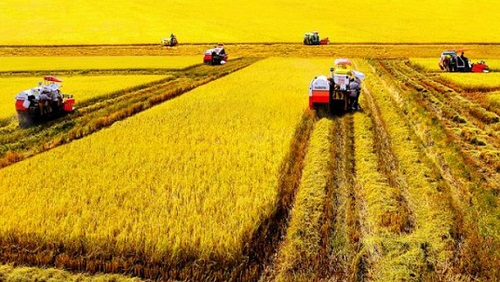
\includegraphics[scale=.5]{Chapter 1/image chapter 1/canhdongMauLon.jpg}
	\caption[Cánh đồng mẫu lớn ở An Giang]{Cánh đồng mẫu lớn ở An Giang}
\end{figure}
\subsubsection{Nông nghiệp thông minh được áp dụng trên thế giới}
\begin{itemize}
	\item Các cỗ máy siêu lớn cho các cánh đồng quy mô khổng lồ 
	\item Canh tác nhà kính: là biện pháp tối ưu nhằm kiểm soát điều kiện tự nhiên gây ảnh hưởng đến cây trồng, bảo vệ cây khỏi sâu, bệnh hại không mong muốn.
	\item Công nghệ đèn LED: giúp cây hấp thụ tối đa lượng ánh sáng cần thiết cho sự sinh trưởng và phát triển.
	\item Tế bào quang điện: được xem như mặt trời nhân tạo, giúp tối ưu hóa không gian.
	\item Thiết bị không người lái và vệ tinh: khảo sát địa hình, tăng độ chính xác quản lý các dữ liệu của trang trại.
	\item Sử dụng robot nông nghiệp, drone nông nghiệp: giảm thiểu sức lao động của con người, được áp dụng ở rất nhiều các quốc gia trên thế giới. 
	\item Công nghệ tài chính phục vụ trang trại:  xây dựng mô hình quản lý chuẩn,quảng bá sản phẩm của nông trại ra với thị trường bên ngoài.
\end{itemize}
\begin{figure}[H]
	\centering
	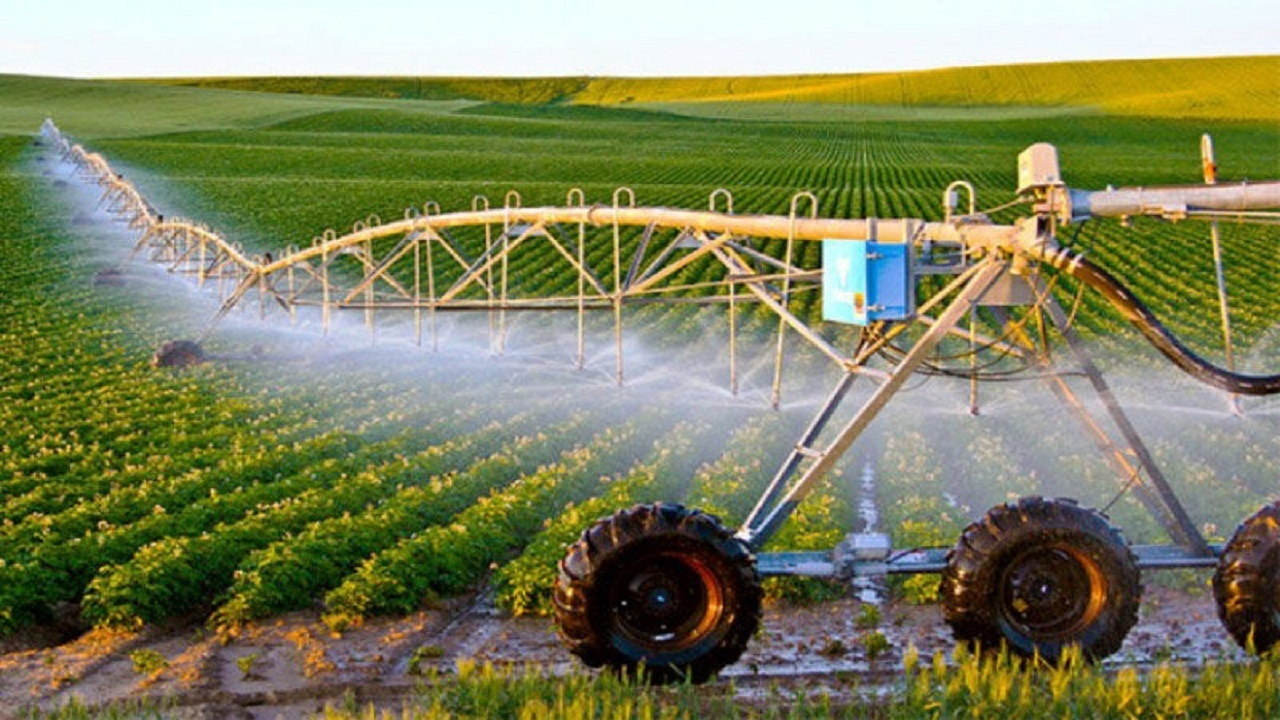
\includegraphics[scale=.3]{Chapter 1/image chapter 1/tuoitieu.jpg}
	\caption[Trang trại công nghiệp công nghệ cao trên thế giới]{Trang trại công nghiệp công nghệ cao trên thế giới}
\end{figure}
\indent Nền nông nghiệp công nghệ đứng đầu thế giới phải nói đến nông nghiệp Israel phát triển ở trình độ cao. Bất chấp bất lợi về địa lý, khí hậu, thiếu nước, phần lớn diện tích là sa mạc không thích hợp cho nông nghiệp. Nhưng bằng sự cố gắng không ngừng Israel đã vươn đứng đầu thế giới về công nghệ và là nhà máy sản xuất nông sản lớn của thế giới.
\begin{figure}[H]
	\centering
	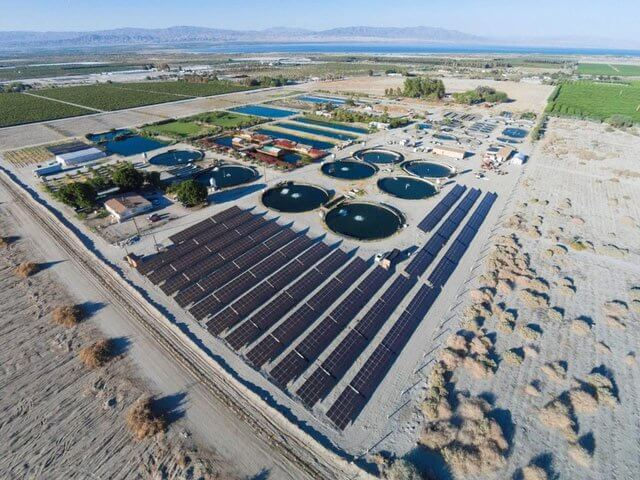
\includegraphics[scale=.6]{Chapter 1/image chapter 1/Israel.jpg}
	\caption[Nhà kính giữa sa mạc của Israel]{Nhà kính giữa sa mạc của Israel}
\end{figure}
\indent Những nền nông nghiệp hàng đầu thế giới đều tập trung vào công nghệ cao và chuyên môn hóa hoàn toàn không phụ thuộc vào địa lý và điều kiện tự nhiên. 
\begin{itemize}
	\item Nhật Bản bắt đầu với nền nông nghiệp trồng lúa tuy nhiên hiện nay nổi tiếng với phòng thí nghiệm siêu sạch trồng xà lách ăn ngay sau khi thu hoạch. 
	\item Hà Lan với hơn 1/3 diện tích thấp hơn mực nước biển, tình trạng nhiễm mặn còn nặng hơn cả đồng bằng sông Cửu Long. Bằng công nghệ cao tập trung đặc khu trồng hoa thu về vài trăm triệu USD mỗi năm và thu hút khách tham quan.
	\item Mỹ với chính sách phát triển nông nghiệp, cơ chế hóa máy móc giảm thiểu sức lao động khi sản xuất trên những nông trại rộng lớn. Không khó để thấy nông dân Mỹ ngồi ca-bin gắn máy điều hòa đi cày xới đất, hay thu hoặc cây trồng. Việc phun thuốc trừ sâu bệnh hoàn toàn bằng máy bay.
\end{itemize}
\subsubsection{Nông nghiệp thông minh ở Việt Nam 10 năm trở lại đây}
Việt Nam là nước mạnh về nông nghiệp, vị trí địa lý thuận lợi, giàu phù sa, kênh rạch chằng chịt mang lại nguồn nước tưới cho cây trồng, là điều kiện tiên quyết cho sản xuất nông nghiệp. Việt Nam bước đầu đưa công nghệ vào sản xuất, thiết bị phun tưới được kết nối Internet vận hành thông qua điện thoại.\\
\indent Tại Đà Lạt hệ thống nhà lưới trồng rau với ánh sáng đèn LED đang được áp dụng, bước đầu đem lại hiệu quả cao. Ngoài ra Đà Lạt còn đi đầu trong việc xây dựng hệ thống trồng rau thủy canh hoàn toàn tự động, phục vụ cho việc cung cấp nông sản sạch và tham quan du lịch. Các vườn hoa tại đây tưới nước hoàn toàn bằng hệ thống tự động đã được thiết lập sẵn, thiết bị cảm biến cho biết độ ẩm, lượng nước tưới và thời gian tưới.
\begin{figure}[H]
	\centering
	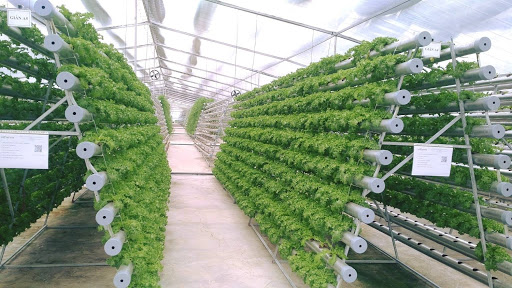
\includegraphics[scale=.5]{Chapter 1/image chapter 1/thuycanh.jpg}
	\caption[Nhà màng trồng rau thủy canh]{Nhà màng trồng rau thủy canh}
\end{figure}
\indent Mô hình khép kín vườn ao chuồng đã được áp dụng từ nhiều năm nay và có bước tiến triển tốt. Hợp tác xã trồng cây theo GAP bao tiêu đầu ra cho nông sản, đảm bảo nguồn gốc thực phẩm cho các siêu thị đã và đang phát triển.\\
\indent Đối với cây lúa, ở nhiều địa phương đã đưa máy móc vào sản xuất cũng như thu hoạch nhằm tối đa năng suất. Ở các hợp tác xã lớn trên cả nước đã tiến hành phun các chế phẩm sinh học trừ sâu, bệnh bằng máy bay tăng độ chính xác và tiến đến sản xuất nông nghiệp hữu cơ.\\
\indent Tuy nhiên, Việt nam vẫn chưa có mô hình nông nghiệp thông minh hoàn chỉnh theo đúng khái niệm. Để có thể phát triển ở Việt Nam, chúng ta cần có giải pháp phù hợp: sự giúp sức của Chính phủ hướng Việt Nam theo nông nghiệp công nghệ cao; tái cơ cấu lại nền nông nghiệp; quy hoạch vùng để phù hợp với loại cây trồng và điều kiện tự nhiên; đào tạo nguồn nhân lực tiếp cận công nghệ cao, hiểu biết và vận hành; mở rộng hợp tác quốc tế cập nhật đổi mới công nghệ từ nước ngoài; xây dựng và quảng bá thương hiệu có sự cạnh tranh trên thế giới.
\subsubsection{Tình hình nghiên cứu mạng LoRa trong nước}
Qua tìm hiểu về tình hình nghiên cứu, trong nước rất ít dự án ứng dụng công nghệ LoRa đưa vào thực tế. Tuy nhiên cũng có rất nhiều dự án, công trình đã và đang được nghiên cứu:
\begin{itemize}
	\item Lê Đình Vương, MSSV 41204661, đề tài luận văn "Thu thập và quản lí dữ liệu thông qua mạng LoRa", Đại học Bách Khoa TP.HCM, tháng 6 năm 2017.
	\item Nguyễn Quốc Anh, MSSV 21300108, đề tài luận văn "Thiết kế hệ thống đo lường chất lượng hồ nuôi tôm sử dụng công nghệ LoRa", Đại học Bách Khoa TP.HCM, tháng 5 năm 2018.
\end{itemize}
\subsubsection{Tình hình nghiên cứu mạng LoRa ngoài nước}
Hiện nay có nhiều cá nhân, công ty nghiên cứu phát hành sản phẩm LoRa mộthay nhiều kênh truyền dựa trên chipset của Semtech. Các công trình nghiên cứu:
\begin{itemize}
	\item Đề tài “A DIY low-cost LoRa gateway” của Giáo sư Phạm Công Đức, trường đại học Paul, Pháp sử dụng chip SX1276 của Semtech với Gateway một kênh truyền.
	\item Module LoRaWan IXM-LPWA-800-16-K9 của Cisco cho các ứng dụng cần công suất thấp, diện tích phủ rộng lớn như tracking vật thể, đo nước hay khí.
\end{itemize}
\subsection{NHIỆM VỤ}
\subsubsection{Mục tiêu đề tài}
Thực hiện truyền dữ liệu nhiệt độ, độ ẩm từ End-node thông qua LoRa về Gateway, Gateway chuyển tiếp dữ liệu thông qua giao thức MQTT về App điện thoại thông minh.\\
\indent Truyền lệnh điều khiển bật/tắt đèn từ App điện thoại thông minh về Gateway thông qua giao thức MQTT, Gateway chuyển tiếp đến End-node thực hiện lệnh thông qua LoRa
\subsubsection{Yêu cầu đề tài}
\begin{itemize}
	\item \textbf{Nội dung 1:} Tìm hiểu module RF UART Lora E32-TTL-100 SX1278 SEMTECH
	\item \textbf{Nội dung 2:} Tìm hiểu MQTT và LoRa
	\item \textbf{Nội dung 3:} Xây dựng App Android
\end{itemize}
\subsubsection{Kế hoạch thực hiện}
\begin{figure}[H]
	\centering
	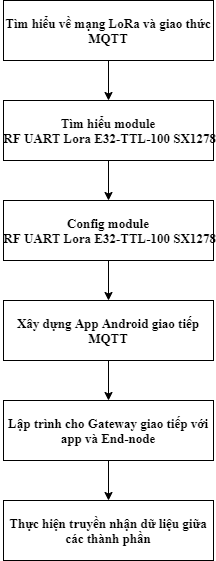
\includegraphics[scale=.5]{Chapter 1/image chapter 1/kehoachthuchien.png}
	\caption[Kế hoạch thực hiện]{Kế hoạch thực hiện}
	\label{hinh11}
\end{figure}
